%% For double-blind review submission
\documentclass[sigplan,10pt]{acmart}\settopmatter{printfolios=true,printccs=false,printacmref=false}
%% For single-blind review submission
%\documentclass[sigplan,10pt,review]{acmart}\settopmatter{printfolios=true}
%% For final camera-ready submission
%\documentclass[sigplan,10pt]{acmart}\settopmatter{}

%% Note: Authors migrating a paper from traditional SIGPLAN
%% proceedings format to PACMPL format should change 'sigplan' to
%% 'acmsmall'.


%% Some recommended packages.
\usepackage{booktabs}   %% For formal tables:
                        %% http://ctan.org/pkg/booktabs
\usepackage{subcaption} %% For complex figures with subfigures/subcaptions
                        %% http://ctan.org/pkg/subcaption
\usepackage{minted}
\usepackage{color,soul}
%% Some recommended packages.
\usepackage{booktabs}   %% For formal tables:
%% http://ctan.org/pkg/booktabs
\usepackage{subcaption} %% For complex figures with subfigures/subcaptions
						%% http://ctan.org/pkg/subcaption


\newcommand{\dz}[1]{{\color{blue}{\it DZ: #1}}}

%% Conference information
%% Supplied to authors by publisher for camera-ready submission;
%% use defaults for review submission.
\acmConference[PPoPP'18]{ACM SIGPLAN Symposium on Principles \& Practice of Parallel Programming}{Feb 24--28, 2018}{Vienna, Austria}
\acmYear{2018}
\acmISBN{978-x-xxxx-xxxx-x/YY/MM}
\acmDOI{10.1145/nnnnnnn.nnnnnnn}
\startPage{1}


%% Copyright information
%% Supplied to authors (based on authors' rights management selection;
%% see authors.acm.org) by publisher for camera-ready submission
%\setcopyright{none}             %% For review submission
\setcopyright{acmcopyright}
%\setcopyright{acmlicensed}
%\setcopyright{rightsretained}
%\copyrightyear{2017}           %% If different from \acmYear


%% Bibliography style
\bibliographystyle{ACM-Reference-Format}
%% Citation style
%% Note: author/year citations are required for papers published as an
%% issue of PACMPL.
%\citestyle{acmauthoryear}  %% For author/year citations
%\citestyle{acmnumeric}     %% For numeric citations
%\setcitestyle{nosort}      %% With 'acmnumeric', to disable automatic
                            %% sorting of references within a single citation;
                            %% e.g., \cite{Smith99,Carpenter05,Baker12}
                            %% rendered as [14,5,2] rather than [2,5,14].
%\setcitesyle{nocompress}   %% With 'acmnumeric', to disable automatic
                            %% compression of sequential references within a
                            %% single citation;
                            %% e.g., \cite{Baker12,Baker14,Baker16}
                            %% rendered as [2,3,4] rather than [2-4].


\begin{document}

\title{FlashR: Parallelize and Scale R for Machine Learning using SSDs}

%% Author information
%% Contents and number of authors suppressed with 'anonymous'.
%% Each author should be introduced by \author, followed by
%% \authornote (optional), \orcid (optional), \affiliation, and
%% \email.
%% An author may have multiple affiliations and/or emails; repeat the
%% appropriate command.
%% Many elements are not rendered, but should be provided for metadata
%% extraction tools.

%% Author with single affiliation.
%\author[1]{\rm Da Zheng}
%\author[1]{\rm Disa Mhembere}
%\author[3]{\rm Joshua T. Vogelstein}
%\author[2]{\rm Carey E. Priebe}
%\author[1]{\rm Randal Burns}
%\affil[1]{Department of Computer Science, Johns Hopkins University}
%\affil[2]{Department of Applied Mathematics and Statistics, Johns Hopkins University}
%\affil[3]{Department of Biomedical Engineering, Johns Hopkins University}

\author{Da Zheng}
\authornote{The work is done when the author was at Johns Hopkins University}          %% \authornote is optional;
\affiliation{
    \institution{Amazon}            %% \institution is required
}

\author{Disa Mhembere}
\affiliation{
    \institution{Dept. of Computer Science, Johns Hopkins University}
}

\author{Joshua T. Vogelstein}
\affiliation{
    \institution{Institute for Computational Medicine,
      Dept. of Biomedical Engineering, Johns Hopkins University}
}

\author{Carey E. Priebe}
\affiliation{
    \institution{Dept. of Applied Math and Statistics, Johns Hopkins University}
}

\author{Randal Burns}
\affiliation{
    \institution{Dept. of Computer Science, Johns Hopkins University}
}

\renewcommand{\shortauthors}{D. Zheng, D. Mhembere, J.T. Vogelstein, C.E. Priebe
    and R. Burns}
%% Paper note
%% The \thanks command may be used to create a "paper note" ---
%% similar to a title note or an author note, but not explicitly
%% associated with a particular element.  It will appear immediately
%% above the permission/copyright statement.
%\thanks{with paper note}                %% \thanks is optional
                                        %% can be repeated if necesary
                                        %% contents suppressed with 'anonymous'


%% Abstract
%% Note: \begin{abstract}...\end{abstract} environment must come
%% before \maketitle command
\begin{abstract}
R is one of the most popular programming languages for statistics and machine
learning, but the R framework alone is relatively slow and unable to scale to large
datasets. The general approach for speeding up an implementation in R is to
implement the algorithms in C or FORTRAN and provide an R wrapper. FlashR takes
a different approach: it parallelizes a large number of matrix functions in
the R \textit{base} package and scales them beyond memory capacity by utilizing
solid-state drives (SSDs) automatically. As such, FlashR parallelizes and scales
existing R code with little/no modification.
FlashR further accelerates parallelized R code by deploying techniques that
reduce data movement between CPU and SSDs:
	\textit{(i)} evaluating all matrix operations lazily,
	\textit{(ii)} performing all matrix operations in a DAG in a single execution
	and with only one pass over data to increase the ratio of computation to I/O,
	\textit{(iii)} performing two levels of matrix partitioning and reordering
	computation on matrix partitions to reduce data movement in the memory hierarchy.
%recycle all memory buffers to reduce memory allocation and CPU cache polution.
We evaluate FlashR on a variety of machine learning and statistics algorithms
on inputs of up to four billion data points. Despite the huge performance
gap between SSDs and RAM, FlashR running on SSDs closely tracks the performance
of FlashR in memory for many machine learning algorithms.
The R code of these machine learning algorithms executed in FlashR
outperforms the in-memory execution of H$_2$O and Spark MLlib by a factor of
$3-20$.
\end{abstract}


%% 2012 ACM Computing Classification System (CSS) concepts
%% Generate at 'http://dl.acm.org/ccs/ccs.cfm'.
\begin{CCSXML}
<ccs2012>
<concept>
<concept_id>10011007.10011006.10011008</concept_id>
<concept_desc>Software and its engineering~General programming languages</concept_desc>
<concept_significance>500</concept_significance>
</concept>
<concept>
<concept_id>10003456.10003457.10003521.10003525</concept_id>
<concept_desc>Social and professional topics~History of programming languages</concept_desc>
<concept_significance>300</concept_significance>
</concept>
</ccs2012>
\end{CCSXML}

%\ccsdesc[500]{Software and its engineering~General programming languages}
%\ccsdesc[300]{Social and professional topics~History of programming languages}
%% End of generated code


%% Keywords
%% comma separated list
\keywords{R, parallel, machine learning, solid-state drives}  %% \keywords is optional


%% \maketitle
%% Note: \maketitle command must come after title commands, author
%% commands, abstract environment, Computing Classification System
%% environment and commands, and keywords command.
\maketitle

\section{Introduction}
% What problem are you going to solve.

The explosion of data and the increasing complexity of data analysis
generate a growing demand for parallel, scalable statistical analysis
and machine learning tools that are simple and efficient.
Simple tools need to be programmable, interactive, and extensible, 
allowing scientists to encode and deploy complex algorithms. 
Successful examples include R, SciPy, and Matlab.  Efficiency dictates that
tools should leverage modern computer architectures, including scalable
parallelism, high-speed networking, and fast I/O from memory and storage.
The current approach for utilizing the full
capacity of modern parallel systems often uses a low-level programming
language such as C and parallelizes computation with MPI or OpenMP.
This approach is time-consuming and error-prone, and requires machine learning
researchers to develop expertise in parallel programming models.
 
% How have others addressed the problem?

While conventional wisdom addresses large-scale data analysis and machine
learning with clusters
\cite{mapreduce,spark,systemml,tensorflow,petuum,graphlab}, recent works
\cite{flashgraph,gridgraph,Matveev17,hotos} demonstrate a single-machine
solution can deal with large-scale data analysis efficiently in a multicore
machine. The advance of solid-state drives (SSDs) allows us to tackle data
analysis in a single machine efficiently at a larger scale and more economically
than possible before. Previous SSD-based graph analysis frameworks
\cite{flashgraph, gridgraph, graphene}
have demonstrated the comparable efficiency to state-of-the-art in-memory graph
analysis, while scaling to arbitrarily large datasets. This work extends
these findings to matrix operations using SSDs for machine learning and
data analysis.
%\dz{we need to say more about the advantage of a single-machine solution
%compare with cluster solutions.}

% Why is it hard?

% What is the nature of your solution?
To provide a simple programming environment for efficient and scalable machine
learning, we present FlashR, an interactive R-based programming framework that
executes R code in parallel and out-of-core automatically. FlashR stores large
vectors and matrices on SSDs and overrides many R functions in the R
\textit{base} package to perform computation on these external-memory vectors
and matrices.
As such, FlashR executes existing R code with little/no modification.
FlashR focuses on optimizations in a single machine (with multiple CPUs and
many cores) and scales matrix operations beyond memory capacity by 
utilizing SSDs.
Our evaluation shows that we can solve billion row, Internet-scale 
problems on a single thick node, which can prevent the complexity,
expense, and power consumption of distributed systems when they are
not strictly necessary \cite{hotos}.

%These machines typically have multiple processors with many CPU cores and
%a large amount of memory. They are also equipped with fast flash
%memory such as solid-state drives (SSDs) to further extend memory capacity.
%This conforms to the node design for supercomputers \cite{Ang14}.

% Why is it new/different/special?

To utilize the full capacity of a large parallel machine, we overcome
many technical challenges to move data from SSDs to CPU efficiently for matrix
computations. Notably, there exist large performance disparities between CPU
and memory and between memory and SSDs, at least an order of magnitude between
every two layers. The ``memory gap'' \cite{Wilkes01} continues to grow, with 
the difference between CPU and DRAM performance increasing exponentially. 
There are also performance differences between
local and remote memory in a non-uniform memory architecture (NUMA), which are prevalent
in modern multiprocessor machines. 
%Even though the I/O
%performance of SSDs has advanced to outperform hard drives by a large factor,
%FDespite advances in SSD I/O performance, 
%they remain an order of magnitude slower than RAM.
%Most matrix computation engines increase data movement,
%because they perform an operation on an entire input matrix prior to moving 
%to the next operation.
% RB -- 
%On the other hand, many analysis tasks are
%data-intensive. Matrix
%formulation further increases data movement between CPU and SSDs because
%a matrix computation framework typically performs an operation
%on the entire input matrices before moving to the next operation.
% As such,
%the performance of the data analysis tasks is usually limited by memory
%bandwidth instead of computing power.

FlashR evaluates expressions lazily and fuses operations aggressively
in a single parallel execution job to minimize data movement. FlashR
builds a directed acyclic graph (DAG) to represent a sequence of matrix
operations. To increase the ratio of computation to I/O, materialization
of any matrix operation in a DAG triggers materialization of all operations
in the DAG. FlashR requires only one pass over the input matrices of
the DAG to perform all operations. FlashR by default keeps only the output
matrices (leaf nodes) of the DAG in memory to have a small memory footprint.
When materializing a DAG, FlashR assigns the same partitions from
different matrices to the same NUMA node
to reduce remote memory access, performs two levels of matrix partitioning
and reorders computation on matrix partitions to reduce data movement
in the memory hierarchy.

% What are it's key features?

We implement multiple machine learning algorithms, including principal component
analysis, logistic regression and k-means, in FlashR. We demonstrate that
with today's fast commodity storage technology, the out-of-core execution of
FlashR achieves performance comparable to their in-memory execution, both
on a large parallel machine and Amazon cloud. Furthermore, FlashR outperforms
the same algorithms in H$_2$O \cite{h2o} and Spark MLlib \cite{spark} by a factor
of $3-20$ in a large parallel machine with 48 CPU cores. In the Amazon cloud,
FlashR using only one fourth of the resources still matches or even outperforms
H$_2$O and Spark MLlib. This suggests that FlashR is a much
more cost-effective solution for large-scale data analysis in the cloud.
FlashR effortlessly scales to datasets with billions
of data points and its out-of-core execution uses a negligible amount of memory
compared with the dataset size. In addition, FlashR executes the R functions
in the R MASS \cite{mass} package with little modification and outperforms
the execution of the same functions in Revolution R Open \cite{rro} by more
than an order of magnitude.

Given its high-level array-oriented programming interface and superior performance,
we argue that FlashR significantly lowers the requirements for writing
parallel and scalable implementations of machine learning algorithms. It also
offers new design possibilities for data analysis clusters, replacing memory
with larger and cheaper SSDs and processing bigger problems on fewer nodes.
FlashR is released as an open-source project at \href{http://flashx.io}{http://flashx.io}.

Our contributions include:
\begin{itemize}
\item We develop an R-based programming framework that executes native R code
in parallel and out of core automatically.
\item We design multiple techniques in our framework to move data from
I/O storage to the CPU cache efficiently and demonstrate that with today's I/O
technology, our SSD-based solution delivers performance approaching that of
in-memory solutions for many machine learning algorithms.
\item We demonstrate that with sufficient system-level optimizations, R code
can easily scale to terabytes of data in a single machine and significantly
outperform optimized parallel machine learning libraries.
\end{itemize}

%\begin{itemize}
%\item identify a set of generalized matrix operations that cover all matrix
%operations in NumPy.
%\item design a set of optimizations for these generalized matrix operations
%to maximize CPU cache hits and reduce I/O access. The optimizations are tailored
%specifically for machine learning.
%\item using SSDs, EM performance matches IM performance and scale to
%Internet-scale datasets.
%\end{itemize}


\vspace{-10pt}
\section{Related Work}
Basic Linear Algebra Subprograms (BLAS) defines a small set of vector and
matrix operations for shared memory. There exist a few
highly-optimized BLAS implementations, such as MKL \cite{mkl}, OpenBLAS
\cite{openblas}, GotoBLAS \cite{Goto} and ATLAS \cite{atlas}. 

Distributed-memory libraries \cite{trilinos, petsc, elemental}
scale to larger matrices. 
These build on BLAS and distribute computation with MPI.
They provide a limited set of predefined matrix operations and
require users to manually parallelize the remaining matrix operations.
%In contrast, FlashMatrix provides a few parallelized GenOps that 
%represent common data access patterns. 
%Each GenOp covers a large number of matrix operations.

Recent works on out-of-core linear algebra \cite{Toledo99, Quintana-Orti12}
focus on redesigning algorithms to achieve efficient I/O access and reduce I/O
complexity. These works are orthogonal to our work and can be adopted to
achieve in-memory performance for these linear algebra routines.

%There are many distributed data processing frameworks.
MapReduce \cite{mapreduce} 
provides a single primitive that takes two user-defined functions. 
% RB not true
%written in low-level programming languages such as C/C++ and Java. 
For matrixes, MapReduce algorithms are inefficient, because they lack
primitives for matrix data access patterns.
Dryad \cite{dryad} and Naiad \cite{naiad} provide more primitives 
that support various data access patterns more efficiently.

Many frameworks that reduce programming complexity have been developed on top of distributed engines.
%Due to complexity of programming in the distributed execution engines, many
%programming frameworks have been developed on top of the distributed execution
%engines. 
Pig Latin \cite{pig} and FlumeJava \cite{flumejava}
provide high-level operations for general data analysis on Hadoop.
SystemML \cite{systemml} has a focus on machine learning. 
DryadLINQ \cite{dryadlinq} expresses data analysis tasks on Dryad. 
%Performance is determined by the underlying distributed execution engines.

The Spark \cite{spark} distributed, in-memory framework
provides a highly-optimized machine learning library (MLlib, \cite{mllib}).
Spark also provides an R programming interface called SparkR.  
We compare FlashMatrix with MLlib; Spark is the most efficient distributed engine.
%, which
%focuses on computation on data frames, a table-like data structure in R.
% DZTODO  what are data frames?

Efforts to parallelize array programming include
Revolution R \cite{rre} and Matlab's parallel computing toolbox, which
offer multicore parallelism and explicit distributed parallelism using MPI and MapReduce. 
Other works focus on implicit parallelization.
Presto \cite{presto} extends R to sparse matrix operations in distributed memory for graph
analysis. Ching et. al \cite{Ching12} parallelizes APL code by
compiling it to C. Accelerator \cite{accelerator} compiles
data-parallel operations on the fly to execute programs on a GPU.


\section{Design}

FlashMatrix is a matrix-oriented programming framework for general data analysis.
This work mainly focuses on dense matrices and scales dense matrix operations
beyond memory capacity by utilizing fast I/O devices,
such as solid-state drives (SSDs), in a non-uniform memory architecture (NUMA).
The implementation and optimization of sparse matrix multiplication is described
in \cite{SEM_SpMM}.
FlashMatrix uses R as its main programming interface and executes R code
automatically in parallel and out of core.

Figure \ref{fig:arch} shows the architecture of FlashMatrix. The core of
FlashMatrix provides a small number of generalized matrix operators (GenOps)
to simplify the implementation and improve the expressiveness of
the framework. The optimizer in FlashMatrix aggressively merges operators to
reduce CPU cache misses and I/O accesses and achieve better parallelization.
FlashMatrix stores large matrices on SSDs through SAFS \cite{safs},
a user-space filesystem for a large SSD array, to fully utilize high I/O
throughput of the SSDs and deploys a set of I/O optimizations to improve
its sequential I/O throughput \cite{SEM_SpMM}.

\begin{figure}
\centering
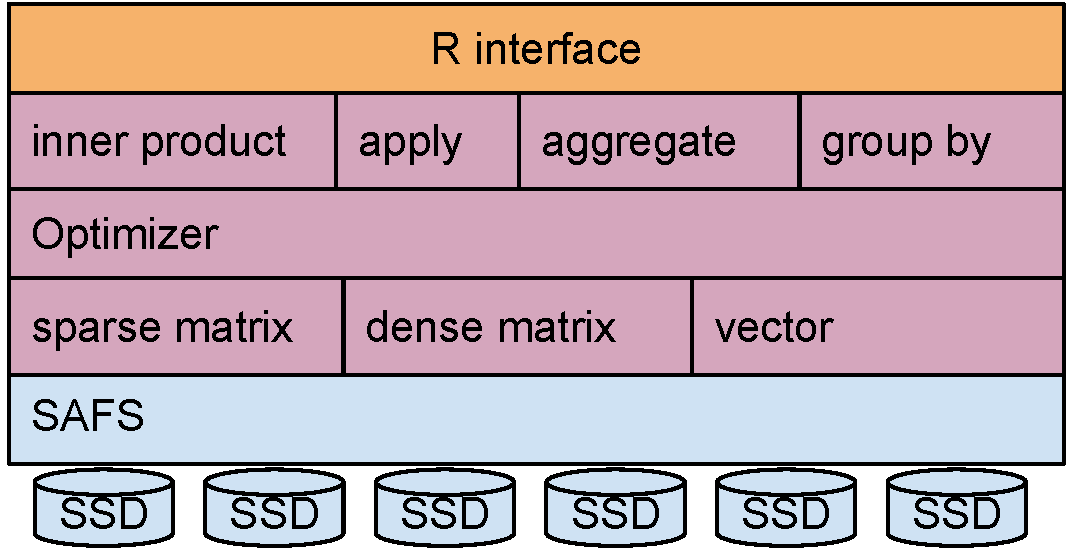
\includegraphics[scale=0.3]{FlashMatrix_figs/architecture.pdf}
\caption{The architecture of FlashMatrix.}
\label{fig:arch}
\end{figure}

FlashMatrix provides a matrix-oriented functional programming interface.
It exposes GenOps in its R interface and reimplements many functions
from the R \textit{base} package with GenOps. The matrices in FlashMatrix
are immutable. Each function operates on one or more matrices and outputs
a new matrix. The functions provided by the R interface are categorized into
seven classes:
\begin{itemize}
	\item The generalized matrix operators (GenOps).
	\item The construction functions that create vectors and matrices of
		the specified size and fill them with specified data (e.g., sequence
		number or random number).
	\item The conversion functions that convert between FlashMatrix matrices and
		R matrices to enable interaction between FlashMatrix and the R framework.
	\item The transformation functions that change the shape of a matrix.
		The commonly used functions include matrix transpose, matrix combination,
		such as \textit{rbind} and \textit{cbind}, and submatrix extraction.
	\item Element-wise operations such as matrix addition and subtraction.
	\item Aggregation operations, such as summation.
	\item BLAS matrix multiplication.
\end{itemize}

%\subsection{SAFS}

%SAFS \cite{safs} is a user-space filesystem for a high-speed SSD array in
%a NUMA machine. It is implemented as
%a library and runs in the address space of its application. It is deployed
%on top of the Linux native filesystem. SAFS was originally designed for
%optimizing small I/O accesses. However, FlashMatrix accesses data in matrices
%sequentially and
%generates much fewer but much larger I/O. Therefore, we provide additional
%optimizations to maximize sequential I/O throughput from a large SSD array.

%The first optimization is to enable polling for I/O to reduce thread context
%switches. On a high-speed SSD array, the latency caused by a thread context
%switch becomes noticeable under a sequential I/O workload and it becomes
%critical to avoid thread
%context switch to gain I/O performance. If the computation in application
%threads does not saturate CPU, SAFS will put the application threads into
%sleep while they are waiting for I/O. This results in many thread context
%switches and underutilization of both CPU and SSDs. To saturate I/O,
%an application thread issues asynchronous I/O to SAFS and poll for I/O
%completion after completing all computation available to it. Polling avoids
%a thread from being switched out during I/O access and effectively maximizes
%I/O throughput of a high-speed SSD array.

%To better support access to many files simultaneously, SAFS stripes data in
%a file across SSDs with a different striping order for each file. Due to
%the sequential I/O workload, FlashMatrix stripes data across SSDs with a large
%block size, on the order of megabytes, to increase I/O throughput and reduce
%write amplification on SSDs \cite{Tang15}. Such a large block size may cause
%storage skew for small files on a large SSD array if every file stripes data
%in the same order. Using the same striping order also causes skew in I/O access.
%Therefore, SAFS generates a random striping order for each file to evenly
%distribute I/O among SSDs. SAFS stores the striping order with a file for
%future data retrieval.

%When accessing a file sequentially from SSDs, we maintain a set of memory buffers
%for I/O access to reduce the overhead of memory allocation.
%We use large I/O to increase I/O throughput. As such, we need to allocate
%a large memory buffer for I/O access.
%The operating system usually allocates a large memory buffer with \textit{mmap()}
%and populates the buffer with physical pages when it is used. It is
%computationally expensive to populate
%large memory buffers frequently. When accessing high-throughput I/O devices,
%such overhead can cause substantial performance loss. Therefore, we keep a set
%of memory buffers allocated previously and reuse them for new I/O requests.

\subsection{Dense matrices}
Dense matrices are the main data types in FlashMatrix. A vector is stored
as a one-column dense matrix. In FlashMatrix, a dense matrix can be stored
physically in memory or on SSDs or represented virtually by a sequence of
computation. FlashMatrix supports dense matrices of different shapes
(Figure \ref{fig:mat}). It specifically optimizes tall-and-skinny matrices
and short-and-wide matrices, and view tall matrices and wide matrices
as groups of tall-and-skinny matrices and short-and-wide matrices, respectively.

\begin{figure}
	\centering
	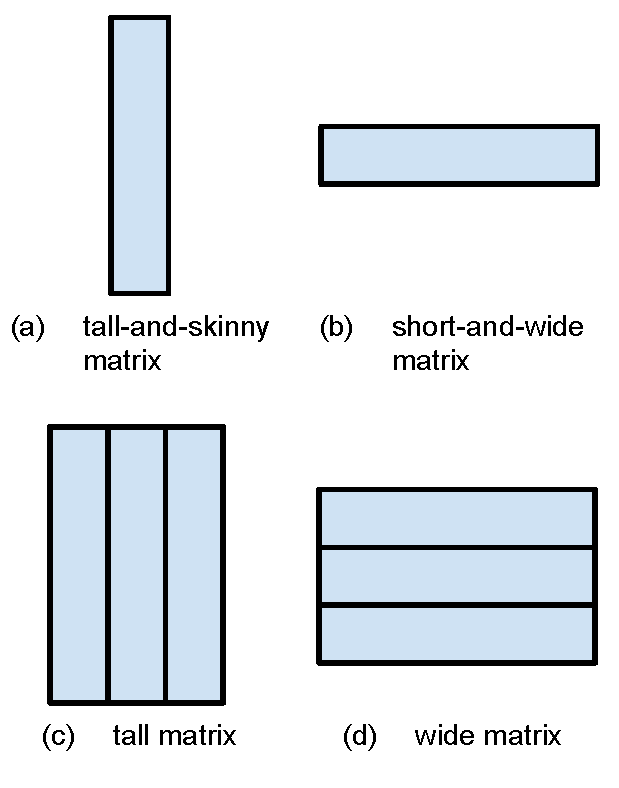
\includegraphics[scale=0.5]{FlashMatrix_figs/matrix.pdf}
	\caption{Dense matrices of different shapes.}
	\label{fig:mat}
\end{figure}

%A matrix has two identifiers: the \textit{matrix identifier} that indicates
%the matrix itself and the \textit{matrix data identifier} that indicates
%the data in the matrix. When a matrix is cloned or transposed, the new matrix
%has a different \textit{matrix identifier} but shares the same
%\textit{matrix data identifier} with the original matrix.

\subsubsection{Tall-and-skinny matrices} \label{sec:tas_mat}

FlashMatrix optimizes for tall-and-skinny (TAS) dense matrices (Figure
\ref{fig:mat} (a)) due to their
frequent occurrence in data analysis. In this field, many data matrices contain
a large number of samples with a relatively few attributes, so 
data matrices are usually tall and skinny. If a data matrix has many
attributes, the first step is often dimension reduction \cite{Jain00}, which
results in a TAS matrix. FlashMatrix specifically optimizes for TAS dense
matrices with tens of columns or fewer. The same optimizations are applied
to short-and-wide matrices (Figure \ref{fig:mat} (b)).

FlashMatrix supports row-major and column-major matrix layout (Figure
\ref{fig:tas_mat}). As such,
we avoid data copy for common matrix operations such as matrix transpose.
Furthermore, each GenOp has its own preferred matrix layout. FlashMatrix
optimizes matrix operations for both data layouts. The layout of an output
matrix is generally determined by a GenOp.

\begin{figure}
	\centering
	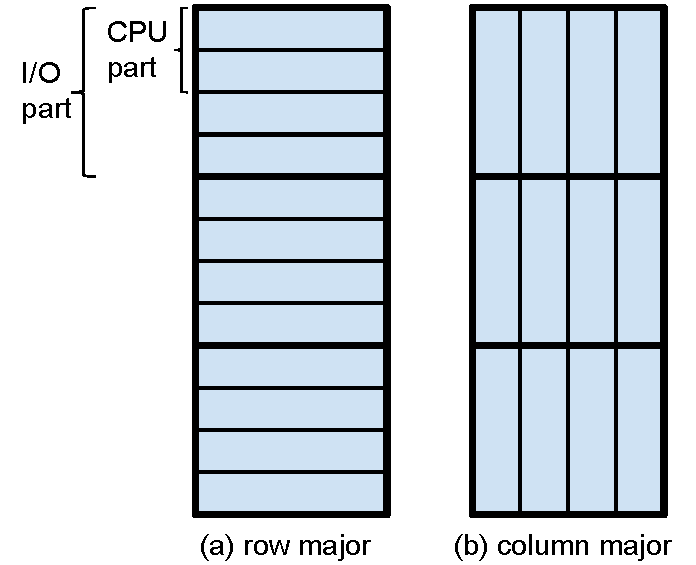
\includegraphics[scale=0.5]{FlashMatrix_figs/dense_matrix.pdf}
	\caption{The format of a tall-and-skinny dense matrix.}
	\label{fig:tas_mat}
\end{figure}

FlashMatrix uses two-level horizontal partitioning on TAS matrices for efficient
data access to SSDs and main memory (Figure \ref{fig:tas_mat}). FlashMatrix
first partitions both in-memory and external-memory TAS matrices horizontally
into I/O-level partitions. All elements in an I/O-level partition are stored
contiguously regardless of the data layout in the matrix. For an in-memory matrix,
the partition size determines the size of contiguous memory required in memory
allocation (see Section \ref{sec:mem}). For an external-memory matrix, each I/O
access reads the entire I/O-level partition, so the partition size determines an I/O
size, usually on the order of megabytes. The number of rows in an I/O-level
partition is always $2^i$. This produces column-major TAS matrices whose data
are well aligned in memory to help CPU vectorization.
We further split an I/O-level partition
horizontally into CPU-level partitions for computation. We use a small
CPU-level partition (on the order of kilobytes) so that it fits in CPU L1/L2
cache to reduce CPU cache misses when evaluating a sequence of matrix
operations (Section \ref{sec:lazy_eval}). FlashMatrix determines the number
of rows in a CPU-level partition based on the number of columns in a matrix.

%\begin{itemize}
%\item NUMA-level partitioning: When a TAS
%matrix is stored in memory, it is partitioned across NUMA nodes to achieve
%data locality and fully utilize memory bandwidth. NUMA-level partitioning
%maps partitions of different vectors/matrices involved in computation
%to the same NUMA node to reduce inter-processor communication. As such,
%the partition size (the number of rows in a partition) is a global parameter
%and is not affected by the number of columns in a matrix.
%\end{itemize}

\subsubsection{Virtual matrices} \label{virt_mat}
In many cases, we do not need to store the data of a matrix physically. Instead,
we compute and generate its data on the fly. \textit{Virtual matrices} store
computation and potentially the reference
to some other matrices required by the computation. A simple example is a matrix
with all elements having the same value. For such a matrix, we only need to store
a single value and construct its matrix partitions during computation.

\textit{Virtual matrices} are essential for lazy evaluation (Section
\ref{sec:lazy_eval}). All GenOps may output \textit{virtual matrices} that
represent the computation results and store only the computation of the GenOps
and the references to the input matrices. This strategy is
essential for both in-memory and external-memory optimizations to improve
performance. It significantly reduces data access to memory and SSDs as well as
memory allocation overhead for creating new matrices.

%\subsubsection{Cached matrix}
%Memory cache is necessary for external-memory matrices on a machine with
%substantial memory.
%Even though SSDs have significantly improved I/O performance, they are still
%an order of magnitude slower than DRAM. Unfortunately, we cannot rely on
%the page cache in SAFS \cite{sa-cache} to buffer some portion of a dense matrix
%because streaming a matrix to memory always evicts existing data in the page
%cache and generates zero cache hits. Therefore, we explicitly cache some portion
%of a dense matrix.

%We store a matrix cache as an in-memory dense matrix.
%To effectively cache data in a dense matrix, we store a tall matrix in
%column-major and cache the first few columns; we store a wide matrix in row-major
%and cache the first few rows. As such, when computation requests an I/O-level
%partition of a matrix, we only need to issue a single I/O request to read
%the remaining columns or rows to reconstruct the I/O-level partition.

%We use a write-through policy for the matrix cache. As such, even when part of
%a dense matrix is cached, we keep a complete copy of the dense matrix on SSDs.
%The benefit of a write-through policy is to overlap computation and I/O when
%a dense matrix is created and avoid I/O latency when removing the cache.

\subsubsection{A group of dense matrices} \label{sec:mat_group}
FlashMatrix represents a tall matrix with many columns with a group of
tall-and-skinny matrices and a wide matrix with a group of short-and-wide
matrices (Figure \ref{fig:mat} (c) and (d)). We construct a special
\textit{virtual matrix} to represent
a group of dense matrices. To take advantage of the optimizations on matrix
operations on TAS matrices, we decompose a matrix operation on a group of
matrices into operations on individual matrices in the group (Section
\ref{sec:group_op}).
Coupled with the two-level partitioning on TAS matrices, this strategy enables
2D-partitioning on a dense matrix and each partition fits in main memory
or CPU cache.

%\begin{figure}
%	\centering
%	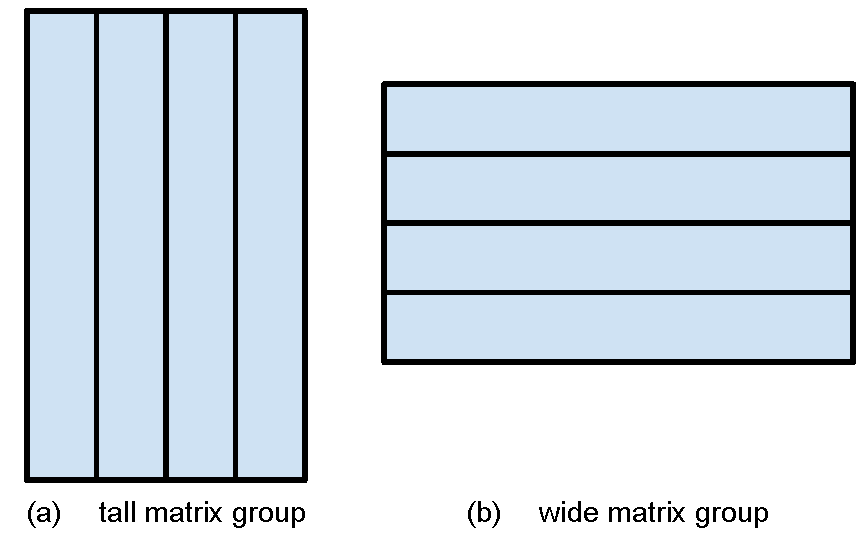
\includegraphics[scale=0.5]{./matrix_group.pdf}
%	\caption{A group of matrices to form a tall matrix with many columns (a)
%	and a wide matrix with many rows (b).}
%	\label{fig:mat_group}
%\end{figure}

%A group of matrices should be stored in a single SAFS file to reduce the number
%of SAFS files.

%append an element to a vector can be implemented as physically appending the element
%to the vector. The result vector becomes the new vector, and the original vector
%becomes the sub-vector of the new vector.

\subsection{Generalized computation operations} \label{sec:genop}
To improve generality and simplify the implementation, FlashMatrix provides
only four generalized operators (GenOps) on matrices: \textit{inner product},
\textit{apply}, \textit{aggregation} and \textit{groupby}. Each operator
represents a data access pattern and accepts some functions as additional
arguments that define computation
on individual elements in matrices (Section \ref{sec:vudf}).

\textit{Inner product} is a generalized matrix multiplication. It replaces
multiplication and addition in matrix multiplication with two functions.
We define many operations with inner product. For example, we use inner product
to compute various pair-wise distances, such as Euclidean distance and Hamming
distance, between data points. For dense matrices, we mainly focus on
optimizing two cases: inner product of a wide matrix and a tall matrix (\textit{inner\_prod\_wide}) and inner product of a tall matrix and a small
matrix (\textit{inner\_prod\_tall}). It is impractical to
materialize inner product of a large tall matrix and a large wide matrix owing
to space complexity. This holds for all matrix algebra frameworks.
%Common
%practice transforms computation that requires this form of inner product to
%the other two forms to reduce space complexity \cite{}.
%Even though we can implement matrix multiplication with inner product,
When evaluating an inner product expression, FlashMatrix uses the BLAS 
implementation of matrix multiplication for floating-point matrices.
This achieves the speed and precision required by
numeric libraries, such as eigensolvers \cite{anasazi, FlashEigen}.

\textit{Apply} is a generalized form of element-wise operations and has
multiple variants. The simplest variant (\textit{sapply}) is
an element-wise unary operation. We use it to implement many unary
operations such as negation, square root or element type casting
on a matrix. The second variant (\textit{mapply}) is an
element-wise binary operation. We use it to implement many binary
matrix operations such as matrix addition and subtraction. The third
(\textit{mapply\_row}) and the fourth variants (\textit{mapply\_col}) perform element-wise
binary operations on the input vector with every row or column of the input
matrix and output a matrix with the same shape as the input matrix.
%Although
%\textit{mapply\_row} and \textit{mapply\_col} can also be implemented by
%replicating the input vector to create a matrix and applying \textit{mapply}
%on the input matrix and the created matrix, \textit{mapply\_row} and
%\textit{mapply\_col} avoid CPU cache polution to improve performance.

\textit{Aggregation} takes multiple elements and outputs a single element.
It has three variants on a matrix. The first variant (\textit{agg})
aggregates over all elements on a matrix, e.g., matrix summation. The second
(\textit{agg\_row}) and the third variants (\textit{agg\_col})
compute aggregation over each individual row or column. \textit{rowSums}
and \textit{colSums} in R are examples.

\textit{Groupby} on a matrix groups rows (\textit{groupby\_row}) or columns
(\textit{groupby\_col}) of a matrix based on a vector of categorical values
and performs aggregation on the rows or
columns associated with the same categorical value. Matrix \textit{groupby}
is used in classification and clustering algorithms that compute
aggregation on the data points in a class or in a cluster.

\subsection{Vectorized user-defined function} \label{sec:vudf}
GenOps take functions that define computation on individual elements.
Computing on each element individually would
result in significant function call overheads. Instead, all of
the GenOps take vectorized user-defined functions (VUDFs) that operate on
a vector of elements instead of an individual element. By transforming
the operations on individual elements to the ones on a vector, we amortize
the overhead of function calls significantly.
%GenOps accept the pointers to VUDFs at runtime to support
%dynamic programming languages such as R.

We balance the amortization of function call overhead and CPU cache misses.
To reduce latency of accessing data in VUDFs,
the input data has to be small enough to fit in the CPU L1 cache. On the
other hand, passing a longer vector to a VUDF amortizes the overhead of
function calls more aggressively. We use 128 as the maximum length of
the input vector of a VUDF. %Futher increasing the length does not have
%noticeable performance improvement.

We have three types of VUDFs to support the GenOps in FlashMatrix. Each VUDF
type may have multiple forms to allow GenOps to transform operations to
increase the length of an input vector to a VUDF and reduce function call
overhead.
\begin{itemize}
	\item A \textit{unary} VUDF (\textit{uVUDF}) takes a vector
		as input and outputs a vector of the same length.
	\item A \textit{binary} VUDF has three forms: the first form (\textit{bVUDF1}) 
    takes two vectors of the same length and outputs
		a vector of the same length as the input vectors; the second form (\textit{bVUDF2}) 
    takes a vector as the left argument and a scalar
		as the right argument and outputs a vector with the same length as
		the input vector; the third form (\textit{bVUDF3}) takes a scalar
		as the left argument and a vector as the right argument and outputs
		a vector. The second and third forms support non-commutative binary
		operations such as division and subtraction.
	\item An \textit{aggregation} VUDF consists of two functions:
		\textit{aggregate} and \textit{combine}. Both functions may have two
		forms: the first one (\textit{aVUDF1}) takes a vector and
		outputs a scalar; the second one (\textit{aVUDF2}) takes
		two vectors of the same length and outputs a vector. For many
		aggregation VUDFs such as summation, \textit{aggregate} and
		\textit{combine} are the same and have both \textit{aVUDF1} and
		\textit{aVUDF2} forms. For some aggregation such as \textit{count},
		\textit{aggregate} and \textit{combine} are different.
\end{itemize}

Figure \ref{fig:DAG} shows an example of using GenOps and VUDFs to compute
standard deviation on a matrix with missing values, a common computation in R.
Standard deviation is computed with the following
formula: $\sigma = \sqrt{E[X^2] - (E[X])^2}$, where $X$ is the input matrix and
$E[X]$ is the mean of the matrix $X$. In the presence of missing values, we
need to exclude the missing values from the matrix. The first step is to apply
$sapply$ with the unary VUDF $sq$ to compute $X^2$ and apply $sapply$ with
the unary VUDF $isna$ to test which elements are missing values. The second
step is to apply $mapply$ with the binary VUDF $ifelse0$ on $X$ and $isna.X$
to replace missing
values in $X$ with 0 and on $X^2$ and $isna.X$ to replace missing values in
$X^2$ with 0. The third step is to apply $agg$ with $+$ to compute summation
of $X$, $X^2$ and $isna.X$. Eventually, we compute the mean of $X$ and
$X^2$ and the standard deviation, excluding missing values.

FlashMatrix provides many commonly used VUDFs. These VUDFs wrap
basic operations built in many programming languages and libraries. For example,
FlashMatrix provides arithmetic operations (\textit{addition} and
\textit{subtraction}), relational operations (\textit{equal to} and
\textit{less than}), logical operations (\textit{logical AND} and
\textit{logical OR}), as well as commonly used math functions (absolute value and square root). 
FlashMatrix also provides a set of VUDFs to
cast primitive element types.

For each basic operation, FlashMatrix provides multiple VUDF
implementations to support different element types. To reduce the number
of binary VUDF implementations, FlashMatrix only provides the ones that take
two input arguments of the same type. If a GenOp gets two matrices with different
element types, it first casts the element type of one matrix to match
the other. %Type casting follows the usual arithmetic conversions \cite{}
%commonly seen in many programming languages.
Type casting operations are
implemented with \textit{sapply} and are performed lazily.

FlashMatrix allows programmers to extend the framework by registering new VUDFs.
Like built-in VUDFs, a new VUDF needs to provide multiple
implementations to support different element types; based on the type of
the VUDF, it may need to provide different forms as described above.
FlashMatrix currently requires a VUDF to be implemented with C/C++.

We use CPU vector instructions such as AVX \cite{avx} to accelerate
the computation in a VUDF. The current implementation of FlashMatrix heavily
relies on auto-vectorization of a compiler, such as GCC, to vectorize
computaion. FlashMatrix provides hints and
transforms code to help auto-vectorization. For example, a VUDF in FlashMatrix
frequently operates on vectors with data aligned in memory and of
the length defined at compile time, so we inform the compiler of the data alignment
and the vector length. Some compilers do not automatically vectorize
aggregation operations well. In this case, we manually create a small vector of reduction
variables, flatten the loop and transform the original aggregation operation
into aggregation onto the vector of reduction variables to help auto-vectorization.

\subsection{Lazy evaluation} \label{sec:lazy_eval}
FlashMatrix evaluates matrix operations lazily. Evaluation of individual
matrix operations results in significant data movement between CPU and SSDs
as well as frequent memory allocation.
Lazy evaluation enables matrix operation fusion to minimize data movement,
reduce memory allocation and improve parallelization \cite{Ching12}.

\begin{figure}
	\centering
	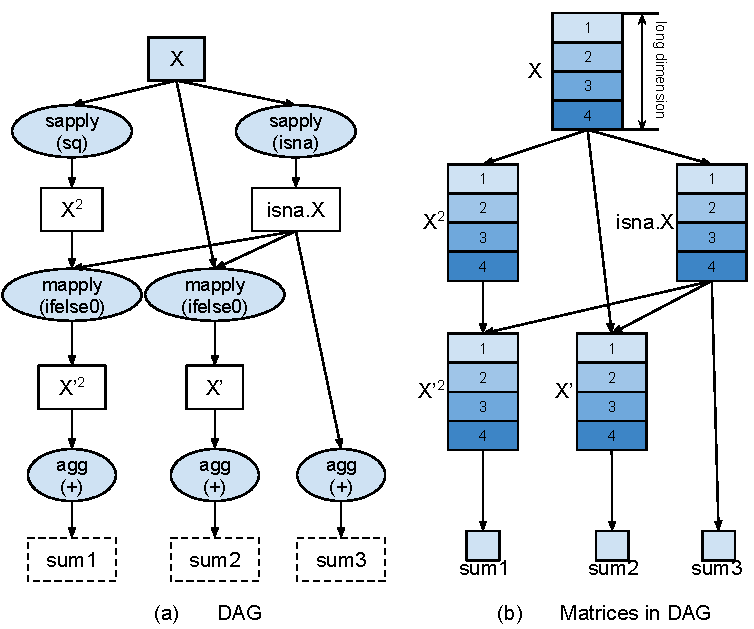
\includegraphics[scale=0.7]{FlashMatrix_figs/sd.pdf}
	\caption{A directed acyclic graph of computing standard deviation on
	a matrix with missing values.}
	\label{fig:DAG}
\end{figure}

FlashMatrix constructs a directed acyclic graph (DAG) to represent a sequence
of matrix operations evaluated lazily (Figure \ref{fig:DAG} (a)). A lazily
evaluated GenOp outputs a \textit{virtual matrix} to capture matrix computation
and the input matrices. A
DAG comprises a set of \textit{virtual matrix} nodes (shown as rectangles)
and computation nodes (shown as ellipses). We refer to the input matrices of
a computation node as the parent matrices and the output matrix as the child matrix.
The computation nodes may contain some immutable computation state, such as
scalar variables and small matrices involved in the matrix computation.
A matrix node can be used by multiple computation nodes as
an input matrix. Although the \textit{virtual matrices} do not need to have
the same shape, FlashMatrix requires all \textit{virtual matrices} in a DAG
to have the same \textit{long dimension} (Figure \ref{fig:DAG} (b)) to
simplify evaluation and data flow of a DAG (a \textit{long dimension}
refers to the matrix dimension with the larger size).

FlashMatrix allows lazy evaluation on all GenOps. There are two types of GenOps
in a DAG. The first type, such as \textit{sapply} and \textit{mapply}, generates
matrices with the same \textit{long dimension} size as the input matrices.
The second type, such as \textit{agg} and \textit{groupby}, generates matrices
with different \textit{long dimension} sizes. The output matrices of the first
type of GenOps can be easily connected to other nodes in a DAG. Any computation
that %changes the long dimension
uses the output matrices of the second type of GenOps
cannot be connected to the same DAG.  We refer to these output matrices as
\textit{sink matrices}.

To enable lazy evaluation, all matrices in FlashMatrix are immutable and every
matrix operation generates a new matrix. As such, materialization of
\textit{virtual matrices} always generates the same result. FlashMatrix
garbage collects a matrix when there are no references to it.

\subsection{Matrix materialization} \label{sec:materialize}
Lazy evaluation postpones computation in matrix operations, but we eventually
have to materialize some \textit{virtual matrices} to perform actual computation.

FlashMatrix can materialize any \textit{virtual matrix} in a DAG and
can materialize multiple \textit{virtual matrices} together. Typically, we
materialize only \textit{sink matrices} in a DAG. In the example shown in
Figure \ref{fig:DAG}, we materialize the three \textit{sink matrices} together
to reduce data movement in the memory hierarchy. Many iterative algorithms need
to materialize some non-\textit{sink matrices} in a DAG to avoid redundant
computation and I/O if these non-\textit{sink matrices} are used across
iterations. FlashMatrix allows programmers to set a flag on the
non-\textit{sink matrices} to inform FlashMatrix to save materialized data
of these matrices to memory or SSDs during computation.

We partition matrices on a DAG in the \textit{long dimension} for materialization
and parallelization (Figure \ref{fig:DAG} (b)). All \textit{virtual matrices}
except \textit{sink matrices} on a DAG have the same \textit{long dimension}
size. To simplify materialization, they all share the same partition size in
the \textit{long dimension}.
As such, a partition $i$ of a \textit{virtual matrix} only requires data from
partitions $i$ of the parent matrices and FlashMatrix materializes partitions
in a matrix independently. %By default, FlashMatrix discards data in a partition
%immediately once the data is used by all children matrices.
%Owing to the storage scheme for
%in-memory matrices, the data of all in-memory matrices in a partition are stored
%on the same NUMA node to minimize remote memory access.
%A \textit{sink matrix} is an output of some form of aggregation on its parent matrix.
When materializing a \textit{sink matrix}, each thread computes partial
aggregation results independently on the partitions of the parent matrix
assigned to the thread. In the end of computation, FlashMatrix merges
the partial aggregation results to construct the \textit{sink matrix}.

%\textit{sink matrices} are usually small and are materialized in memory.
%For example, \textit{agg\_row} on a wide matrix and
%\textit{agg\_col} on a tall matrix outputs a vector. The maximal length of
%the vector is $\sqrt{N}$, where $N$ is the number of elements
%in the input matrix. As such, we can always keep it in memory. For most of machine
%learning and data analysis tasks, the output matrix of the inner product of
%a wide matrix with a tall matrix is usually small and is by default kept
%in memory because the long dimension of these matrices is usually much larger
%than the short dimension in these tasks.

FlashMatrix takes advantage of the two-level
partitioning on dense matrices to reduce data movement between SSDs and CPU.
It assigns I/O-level partitions (Section \ref{sec:tas_mat}) to a thread as
computation tasks for parallelization. We choose a relatively small partition
size to balance the overhead of accessing a partition, skew
and memory consumption. A thread further splits an I/O-level partition into
CPU-level partitions at run time and materializes one CPU-level partition at
a time. After materializing a CPU-level partition, the thread passes the partition
to the subsequent operation in the DAG, instead of materializing the next CPU-level
partition in the same matrix. A CPU-level partition is sufficiently small
to fit in the CPU cache so that the partition still resides in CPU cache when
the subsequent operation consumes it. This significantly reduces data movement
between CPU and memory.
%In a DAG, a matrix may be
%required by multiple GenOps. As such, each matrix always buffers one materialized
%CPU-level partition in each thread to avoid redundant computation.
%\dz{We need to identify transpose of a matrix.}

%FlashMatrix uses a global task scheduler to assign tasks to threads dynamically
%for load balancing and I/O merging. However, SSDs require large
%writes to achieve sustainable write throughout and reduce write amplification
%\cite{}. As such, FlashMatrix delays writing the materialized partitions to
%SSDs and merge multiple materialized partitions into a single write because
%the global task scheduler assigns consecutive partitions to threads.

%To keep data in CPU cache as long as possible, we reuse the memory buffers
%to reduce the number of memory buffers used in the computation and avoid CPU
%cache polution.

\subsection{Memory management} \label{sec:mem}
FlashMatrix manages large memory allocation itself to reduce overhead.
In-memory matrix creation and I/O access to matrices on SSDs require large memory
allocation. The functional programming interface of FlashMatrix leads to more
frequent memory allocation, because each matrix operation generates a new matrix. 
Large memory allocations are expensive in Linux because Linux uses \textit{mmap}
to allocate large memory and relies on page faults to populate the memory.
Frequent page faults prevent computation from fully utilizing CPUs in a large
parallel machine and cause significant performance degradation.

\begin{figure}
	\centering
	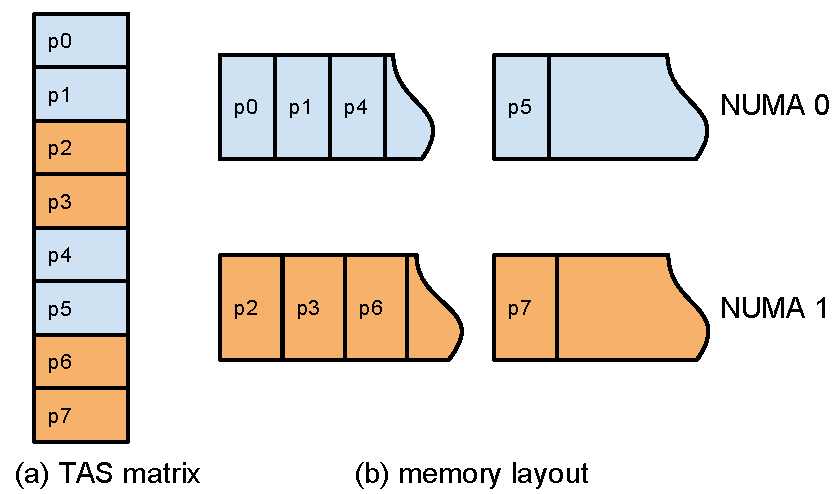
\includegraphics[scale=0.5]{FlashMatrix_figs/matrix_mem.pdf}
	\caption{Memory layout of a tall-and-skinny dense matrix.}
	\label{fig:mat_mem}
\end{figure}

FlashMatrix stores an in-memory matrix in fixed-size memory chunks and
recycles memory chunks to reduce memory allocation overhead (Figure
\ref{fig:mat_mem}). FlashMatrix requires only an I/O-level partition to
be stored in contiguous memory. As long as a memory chunk is sufficient
to store an I/O-level partition, FlashMatrix can store a matrix in a set
of fixed-size memory chunks. The size of a memory chunk is a global parameter
and is the same for all matrices. As such, FlashMatrix reuses memory chunks
allocated for matrices of different shapes. 
%In practice, the memory chunk size
%may not be divisible by an I/O-level partition size. Therefore, the 
We choose the memory chunk
size to be much larger than the I/O-level partition size to increase
memory utilization. We use 64MB as the default memory chunk size.

FlashMatrix maintains per-thread memory buffer pools for accessing I/O-level
partitions of a matrix on SSDs. These memory buffers have the same size as
I/O-level partitions, which are in the order of megabytes to maximize I/O
throughput of an SSD. Because all partitions of a matrix have the same size,
the memory buffers are reused.

\subsection{Implementation of GenOps with VUDF}

GenOps invoke VUDFs on the elements of CPU-level partitions intelligently
to increase the length of vectors passed and to reduce the overhead of
function calls. Different GenOps choose different
forms of VUDFs based on the data layout and the shape of the input matrices.

Some GenOps invoke VUDFs on the elements of matrices efficiently regardless of
data layout and matrix shape.
For example, \textit{sapply} and \textit{mapply} only require
the input matrices and the output matrix to have the same data layout. For tall
column-major matrices and wide row-major matrices, each CPU-level partition has
long columns and long rows, respectively. These GenOps invoke a VUDF
on the long columns and rows. For tall row-major matrices and wide column-major
matrices, all rows and columns in a CPU-level partition are stored in a single
piece of memory. These GenOps invoke a VUDF only once on all
elements in a partition. %A similar strategy is applicable to \textit{agg}.

Most of the GenOps require a matrix with a specific data layout to reduce
function call overhead.
Many of the GenOps favor the column-major order for a tall-and-skinny matrix
and the row-major order for a short-and-wide matrix. These data layouts increase
the length of a vector passed to a VUDF and align data in memory. For example,
the column-major order ensures that each column in a partition of a tall matrix
is aligned in memory, regardless of the number of columns in the matrix. A GenOp,
such as inner product, converts the data layout of a CPU-level partition to
the preferred layout if an input matrix does not have the preferred layout.
%Because a CPU-level partition fits in the CPU cache, data layout conversion
%does not increase data access to main memory. 

Given a matrix with the preferred data layout, a GenOp selects different forms
of a VUDF automatically based on the shape of the input matrix. For example,
for a tall column-major matrix, \textit{mapply\_col} invokes the \textit{bVUDF1}
form of the binary VUDF on a column from the input matrix and the input vector;
for a wide row-major matrix, \textit{mapply\_col} invokes the \textit{bVUDF2}
form on a row from the input matrix and an element from the vector. We apply
the similar strategy to other GenOps. When applying \textit{inner\_prod\_tall}
on a tall column-major matrix, FlashMatrix uses the \textit{bVUDF2} form of
the first VUDF to computes the outer product of a column from the left matrix
and a row from the right matrix, and uses the \textit{aVUDF2} of the second VUDF
to compute the final result. Because \textit{inner\_prod\_tall} operates on
a CPU-level partition, all intermediate results in the computation reside
in CPU cache. \textit{inner\_prod\_wide} invokes the
\textit{bVUDF1} form of the first VUDF on a row from the left matrix and a column
from the right matrix, and invokes the \textit{aVUDF1} form of the second VUDF
on the output from the first VUDF to compute an element in the output matrix for
the input partitions.

%Both \textit{agg\_row} and \textit{agg\_col} work better on the preferred data
%layout if the aggregation VUDF has the same \textit{aggregate} and \textit{combine}
%function with both \textit{aVUDF1} and \textit{aVUDF2} forms. For these aggregation
%VUDFs, we can transform \textit{agg\_row} on a column-major matrix to applying
%\textit{aVUDF2} to columns of a partition. Similar transformation is applied
%to \textit{agg\_col} on a row-major matrix.

%Inner product chooses different forms of VUDFs for input matrices with different
%shapes. The first UDF of inner product is a binary UDF and the second one is an
%aggregation UDF. For the sake of efficiency, inner product requires the second
%UDF to have the same \textit{aggregate} and \textit{combine} function with both
%\textit{aVUDF1} and \textit{aVUDF2} forms.

%Unlike other GenOps, \textit{groupby\_row} and \textit{groupby\_col} are the only
%GenOps that do not favor the column-major order for a tall-and-skinny matrix and
%the row-major order for a short-and-wide matrix. \textit{groupby\_row} sorts
%rows in a partition based on the categorical values associated with each row
%and apply the aggregation VUDF on rows directly.

\subsection{Implementation of GenOps on a group of matrices} \label{sec:group_op}

When applying a GenOp on a group of matrices (Section \ref{sec:mat_group}),
we decompose the computation into multiple GenOps and apply them to individual
matrices in the group if the GenOp supports decomposition. Decomposing computation
to individual matrices reduces memory copies and increases CPU cache hits.
For the GenOps that cannot be decomposed, we combine the individual matrices
on the fly and apply the GenOps on the combined matrix directly.

We apply some of the GenOps to individual matrices directly without
transformation. For example,
\textit{sapply} and \textit{agg} run on individual matrices directly regardless
of the shape and data layout of the matrices. Other GenOps may be applied
to individual matrices directly if the input matrices have certain shape. For
example, we apply \textit{mapply\_col} and \textit{agg\_col} to individual
matrices in a group of tall matrices directly.  Similarly, we apply
\textit{mapply\_row} and \textit{agg\_row} to
individual matrices in a group of wide matrices directly. %\textit{mapply}
%requires the matrices in the two input matrix groups to have the same shape.
%\textit{Groupby\_row} on a \textit{tall matrix group} can be decomposed and
%applied to individual matrices; \textit{groupby\_col} on a \textit{wide matrix group}
%can be decomposed in a similar fashion.

Applying other GenOps to a group of matrices requires transformation. If an aggregation
VUDF provides a \textit{combine} function, applying \textit{agg\_row} to a group of
tall matrices is transformed into two steps: apply the \textit{aggregate} function on
each row of individual matrices and apply the \textit{combine} function on the partial
aggregation results. When applying \textit{mapply\_row} to a group of tall matrices,
we break the input vector into parts to match the number of columns in the individual
matrices in the group and apply \textit{mapply\_row} to individual matrices
separately. We apply the same strategies to \textit{agg\_col} and
\textit{mapply\_col} on a group of wide matrices. 

FlashMatrix decomposes inner product on a matrix group in favor of minimizing
the amount of data written to SSDs (Figure \ref{fig:inner_prod}).
For \textit{inner\_prod\_tall}, we first partition the right matrix vertically
so that the inner product of the left matrix and a vertical partition outputs
part of a final output matrix. The number of vertical partitions determines
the number of runs required to complete the inner product on the group of matrices.
If the left matrix is stored on SSDs, the number of vertical partitions on
the right matrix determines the amount of data read from SSDs. The vertical
partition size determines the output matrix size in each run and affect
the memory size. As such, we need to select the vertical partition size of
the right matrix to balance I/O and memory consumption. We horizontally partition
each vertical partition of the right matrix to further decompose the inner
product. We construct a directed acyclic graph (DAG) to evalute the inner
product lazily (Section \ref{sec:lazy_eval}). Similarly, we partition the right
matrix and make a similar choice to balance I/O and memory consumption for
\textit{inner\_prod\_wide}. We also construct a DAG and lazily evaluate
the computation.

\begin{figure}
\centering
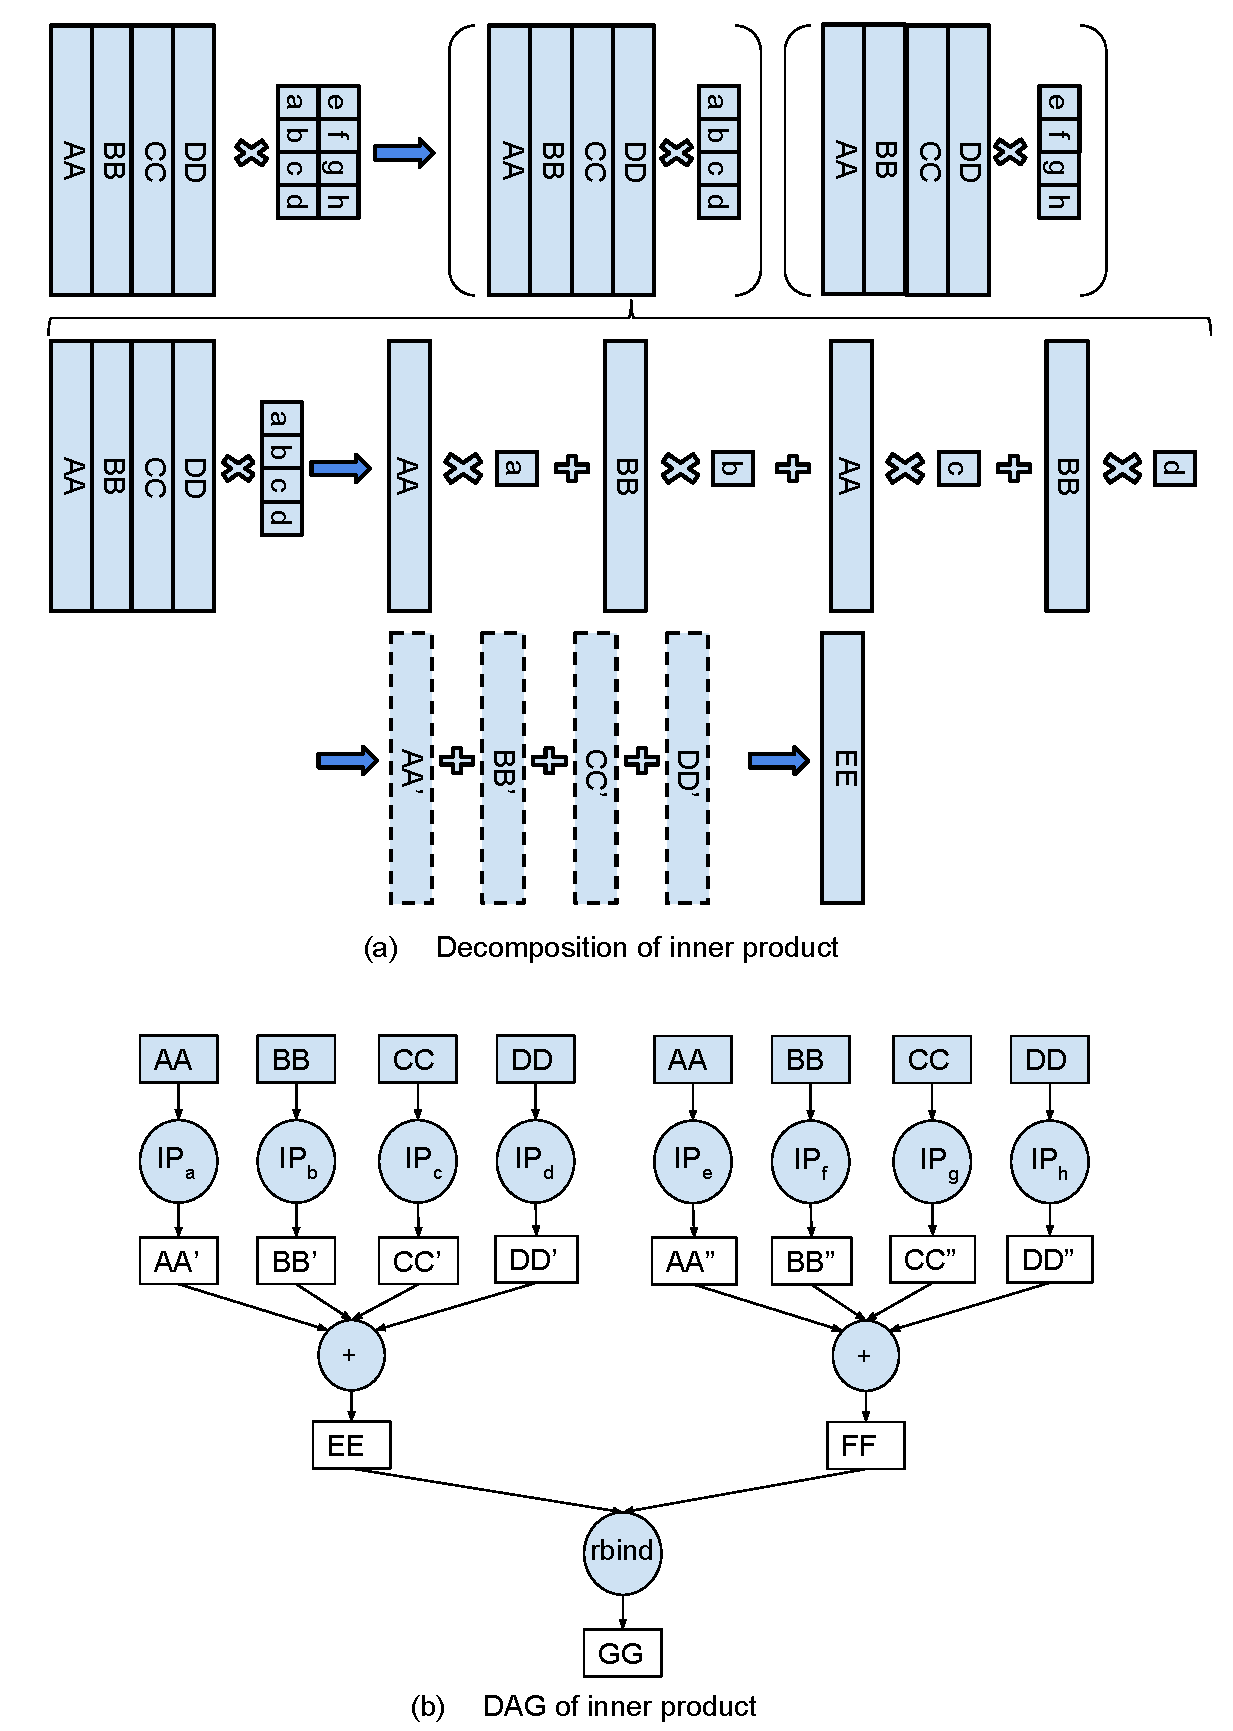
\includegraphics[scale=0.4]{FlashMatrix_figs/inner_prod_tall.pdf}
\vspace{-5pt}
\caption{Decomposition inner product on a group of dense matrix.}
\vspace{-5pt}
\label{fig:inner_prod}
\end{figure}


\section{Experimental evaluation}
We evaluate the efficiency of FlashR on statistics and machine learning
algorithms both in memory and on SSDs. We compare the R implementations of
these algorithms with the ones in two optimized parallel machine learning
libraries H$_2$O \cite{h2o} and Spark MLlib \cite{mllib}. We further use FlashR
to accelerate existing R functions in the MASS package and compare with
Revolution R Open \cite{rro}.

We conduct experiments on our local server and Amazon cloud. The local server
is a large NUMA machine with four Intel Xeon E7-4860 2.6 GHz processors,
each of which has 12 cores, and 1TB of DDR3-1600 memory. The machine is equipped
with 24 OCZ Intrepid 3000 SSDs, which together are capable of 12 GB/s for read
and 10 GB/s for write. We also run FlashR on an EC2 i3.16xlarge instance,
which has 64 virtual CPUs, 488GB of RAM and 8 NVMe SSDs. The NVMe SSDs together
provide 15.2TB of space and up to 16GB/s of sequential I/O throughput.
We run Ubuntu 16.04 and use ATLAS 3.10.2 as the default BLAS library on both
machines.

\subsection{Benchmark algorithms}\label{benchalg}
We benchmark FlashR with some commonly used machine learning algorithms.
These algorithms have various ratios of computation and I/O complexity
(Table \ref{tbl:algs}) to thoroughly evaluate performance of FlashR on SSDs.
Like the algorithms
shown in Section \ref{sec:apps}, we implement these algorithms completely with
the R code and rely on FlashR to execute them in parallel and out-of-core.
We implement these machine learning algorithms in FlashR identically to our
competitors (SparkML and H2O). 

\noindent \textbf{Correlation} computes pair-wise Pearson's correlation
\cite{cor} and is commonly used in statistics.

\noindent \textbf{Principal Component Analysis (PCA)} computes uncorrelated
variables from a large dataset. PCA is commonly used for dimension reduction
in many data analysis tasks. We compute PCA by computing eigenvalues on the Gramian
matrix $A^T A$ of the input matrix $A$.

\noindent \textbf{Naive Bayes} is a classifier that applies Bayes' theorem
with the ``naive'' assumption of independence between every pair of features.
Our implementation assumes data follows the normal distribution.

\noindent \textbf{Logistic regression} is a linear regression model with
categorical dependent variables. We use the LBFGS algorithm \cite{lbfgs}
to optimize logistic regression. In the experiments, it converges when
$logloss_{i-1}-logloss_i < 1e-6$, where $logloss_i$ is the logarithmic loss
at iteration $i$.

\noindent \textbf{K-means} is an iterative clustering algorithm that
partitions data points into $k$ clusters. Its R implementation is illustrated
in Figure \ref{fig:kmeans}. In the experiments, we run k-means to split
a dataset into 10 clusters by default. It converges when no data points
move.

\noindent \textbf{Gaussian mixture models (GMM)} assumes data follows
a mixture of Gaussian distribution and learns parameters of Gaussian mixture
models from data. It typically uses the expectation-maximization (EM)
algorithm \cite{em} to fit the models, similar to k-means. In the experiments,
it converges when $loglike_{i-1} - loglike_i < 1e-2$, where $loglike_i$
is the mean of log likelihood over all data points at iteration $i$.

\noindent \textbf{Multivariate Normal Distribution (mvrnorm)} generates
samples from the specified multivariate normal distribution. We use
the implementation in the MASS package.

\noindent \textbf{Linear discriminant analysis (LDA)} is a linear classifier
that assumes the normal distribution with a different mean for each class
but sharing the same covariance matrix among classes. We use the implementation
in the MASS package with some trivial modifications.

\begin{table}
\begin{center}
\caption{Computation and I/O complexity of the benchmark algorithms. For
	iterative algorithms, the complexity is per iteration. $n$ is the number
	of data points, $p$ is the number of the features in a point, and $k$ is
	the number of clusters. We assume $n > p$.
}
\vspace{-10pt}
\footnotesize
\begin{tabular}{|c|c|c|c|c|}
\hline
Algorithm & Computation & I/O \\
\hline
Correlation & $O(n \times p^2)$ & $O(n \times p)$ \\
\hline
PCA & $O(n \times p^2)$ & $O(n \times p)$ \\
\hline
Naive Bayes & $O(n \times p)$ & $O(n \times p)$ \\
\hline
Logistic regression & $O(n \times p)$ & $O(n \times p)$ \\
\hline
K-means & $O(n \times p \times k)$ & $O(n \times p)$ \\
\hline
GMM & $O(n \times p^2 \times k)$ & $O(n \times p + n \times k)$ \\
\hline
mvrnorm & $O(n \times p^2)$ & $O(n \times p)$ \\
\hline
LDA & $O(n \times p^2)$ & $O(n \times p)$ \\
\hline
%PageRank & $O(nnz + n)$ & $O(nnz)$ \\
%\hline
\end{tabular}
\normalsize
\label{tbl:algs}
\end{center}
\vspace{-10pt}
\end{table}

\subsection{Datasets}\label{sec:data}
We use two real-world datasets with billions of data points (Table \ref{tbl:data})
to benchmark the algorithms above. The Criteo dataset has over four billion data
points with binary labels (click vs. no-click), used for advertisement click
prediction \cite{criteo}. PageGraph-32ev are 32 singular vectors that we computed
on the largest connected component of a Page graph, which has 3.5 billion vertices and
129 billion edges \cite{webgraph}. Because Spark MLlib and H$_2$O cannot process
the entire datasets in a single machine, we take part of the Criteo and
PageGraph-32ev datasets to create smaller datasets.
PageGraph-32ev-sub is the first 336 million data points
of the PageGraph-32ev dataset. Criteo-sub contains the data points collected
on the first two days, which is about one tenth of the whole dataset.

\begin{table}
\begin{center}
\caption{Datasets. All datasets are stored as dense matrices.}
\vspace{-10pt}
\footnotesize
\begin{tabular}{|c|c|c|c|c|}
\hline
Data Matrix & \#rows & \#cols \\
\hline
PageGraph-32ev \cite{webgraph} & 3.5B & 32 \\
\hline
Criteo \cite{criteo} & 4.3B & 40 \\
\hline
PageGraph-32ev-sub \cite{webgraph} & 336M & 32 \\
\hline
Criteo-sub \cite{criteo} & 325M & 40 \\
\hline
\end{tabular}
\normalsize
\label{tbl:data}
\end{center}
\vspace{-10pt}
\end{table}

%\vspace{-8pt}
\subsection{Comparative performance}
%\vspace{-4pt}
We evaluate FlashR against H$_2$O \cite{h2o} and Spark MLlib \cite{mllib} as well
as Revolution R Open \cite{rro} in our local server and in the Amazon cloud.
Before running the algorithms in H$_2$O and MLlib, we ensure that all data are
loaded and cached in memory. When running in the 48 CPU core local server,
all frameworks use 48 threads. When running in the cloud, we compare FlashR
running in one of the largest I/O-optimized instance (i3.16xlarge) with MLlib
and H$_2$O in a cluster with four of the largest general-purpose instances
(m4.16xlarge), which in total has 256 CPU cores, 1TB RAM and 20Gbps network.
All iterative algorithms take the same number of iterations and generate
similar accuracy\footnote{The only exception is the logistic regression in Spark
because we cannot control its number of iterations}.
We also use FlashR to parallelize functions (mvrnorm and LDA)
in the R MASS package and compare their performance with Revolution R Open. We use
Spark v2.0.1, H$_2$O v3.14.2 and Revolution R Open v3.3.2.

\begin{figure}
  \vspace{-5pt}
	\centering
	\footnotesize
	\begin{subfigure}{.5\textwidth}
		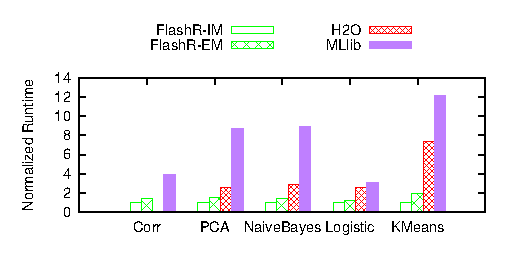
\includegraphics{FlashMatrix_figs/FlashR-vs-dist.eps}
		\caption{In a large parallel machine with 48 CPU cores.}
		\label{perf:para}
	\end{subfigure}

	\vspace{3pt}
	\begin{subfigure}{.5\textwidth}
		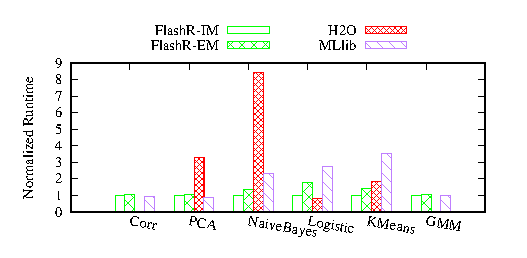
\includegraphics{FlashMatrix_figs/FlashR-vs-dist-EC2.eps}
		\caption{In the Amazon cloud. FlashR-IM and FlashR-EM run on one
			EC2 i3.16xlarge instance (64 CPU cores) and Spark MLlib runs
		on a cluster of four EC2 m4.16xlarge instances (256 CPU cores).}
		\label{perf:cloud}
	\end{subfigure}
	\vspace{-8pt}
	\caption{The normalized runtime of FlashR in memory (FlashR-IM) and
	on SSDs (FlashR-EM) compared with H$_2$O and Spark MLlib. Correlation and GMM
	are not available in H$_2$O. We run k-means and GMM on the PageGraph-32ev-sub
	dataset and all other algorithms on the Criteo-sub dataset.}
	\label{perf:rt}
  \vspace{-10pt}
\end{figure}

FlashR running on SSDs (FlashR-EM) achieves at least half the performance of
running in memory (FlashR-IM), while outperforming H$_2$O\footnote{
H$_2$O develops machine learning algorithms individually and adding
a new algorithm in H$_2$O requires writing it from scratch, which is
a non-trivial task. H$_2$O does not provide implementations for correlation
and GMM, so we do not provide results for these two algorithms.}
and Spark MLlib significantly on all algorithms
(Figure \ref{perf:para}) in the large parallel machine with 48 CPU cores.
When all frameworks run on the same hardware, FlashR-IM achieves 4 to 10 times
performance gain when compared
with MLlib, and 3 to 20 times performance gain when compared with H$_2$O.
All implementations rely on BLAS for matrix multiplication, and H$_2$O
and MLlib implement non-BLAS operations with Java and Scala, respectively.
Spark materializes operations such as aggregation separately. In contrast,
FlashR fuses matrix operations and performs two-level partitioning to
minimize data movement in the memory hierarchy and keeps data in CPU cache
to achieve high memory bandwidth.


We further evaluate the performance of FlashR on Amazon EC2 cloud and compare it
with Spark MLlib and H$_2$O on an EC2 cluster (Figure \ref{perf:cloud}). H$_2$O
recommends
allocating a total of four times the memory of the input data. As such, we use
4 m4.16xlarge instances that provide sufficient memory and computation power for
Spark MLlib and H$_2$O to process the datasets (PageGraph-32ev-sub and Criteo-sub).
Even though Spark MLlib and H$_2$O have four times as much computation power as FlashR,
FlashR still outperforms both distributed machine learning libraries in most algorithms.
Because the NVMes in i3.16xlarge provide higher I/O throughput than the SSDs
in our local server, the performance gap between FlashR-IM and FlashR-EM gets
smaller.

\begin{figure}[b]
  \vspace{-10pt}
	\begin{center}
		\footnotesize
		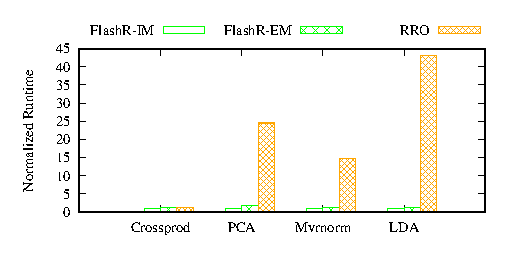
\includegraphics{FlashMatrix_figs/FlashR-vs-RRO.eps}
		\vspace{-10pt}
		\caption{In-memory (FlashR-IM) and out-of-fore (FlashR-EM) FlashR
		compared with Revolution R Open on a data matrix with one million rows
		and one thousand columns when running on the parallel machine with
		48 CPU cores.}
		\label{fig:fmR}
	\end{center}
  \vspace{-15pt}
\end{figure}

FlashR running both in memory and on SSDs outperforms Revolution R Open by more
than an order of magnitude even on a small dataset ($n=1,000,000$ and $p=1000$)
(Figure \ref{fig:fmR}).
Revolution R Open uses Intel MKL to parallelize matrix multiplication. As such,
we only compare the two frameworks with computations that use matrix
multiplication heavily. Both FlashR and Revolution R Open run the mvrnorm
and LDA implementations from the MASS package. For simple matrix operations
such as crossprod, FlashR slightly outperforms Revolution R Open.
For more complex computations, the performance gap between FlashR and
Revolution R increases. Even though matrix multiplication
is the most computation-intensive operation in an algorithm, it is insufficient
to only parallelize matrix multiplication to achieve high efficiency.

\subsection{Scalability}

We show the scalability of FlashR on the billion-scale datasets in Table
\ref{tbl:data}. In these experiments, we run the iterative algorithms on
the datasets until they converge (see their convergence condition in Section
\ref{benchalg}).

\begin{table}
\begin{center}
	\caption{The runtime and memory consumption of FlashR on the billion-scale
		datasets on the 48 CPU core machine. We measure the runtime of
                iterative algorithms when they converge. We run k-means and GMM
		on PageGraph-32ev and the remaining algorithms on Criteo.}
\vspace{-10pt}
\footnotesize
\begin{tabular}{|c|c|c|}
\hline
	& Runtime (min) & Peak memory (GB) \\
\hline
Correlation & $1.5$ & $1.5$ \\
\hline
PCA & $2.3$ & $1.5$ \\
\hline
NaiveBayes & $1.3$ & $3$ \\
\hline
LDA & $38$ & $8$ \\
\hline
% in 23 iterations.
Logistic regression & $29.8$ & $26$ \\
\hline
k-means & $18.5$ & $28$ \\
\hline
GMM & $350.6$ & $18$ \\
\hline
\end{tabular}
\normalsize
\label{tbl:scale}
\end{center}
\vspace{-10pt}
\end{table}

Even though we process the billion-scale datasets in a single machine, none of
the algorithms are prohibitively expensive. Simple algorithms, such as
Naive Bayes and PCA, require one or two passes over the datasets and take
only one or two minutes to complete. Iterative algorithms in this experiment
take about $10-20$ iterations to converge and finish computation quickly.
Even though GMM is a computation-intensive algorithm, it does not take
a prohibitively long time to complete.

FlashR scales to datasets with billions of data points easily when running
out-of-core. All of the algorithms have negligible memory consumption.
The scalability of FlashR is mainly bound by the capacity of SSDs.
Two factors contributes to the small memory consumption: \textit{(i)}
due to lazy evaluation, FlashR only needs to materialize the small matrices
to effectively reduce memory consumption; \textit{(ii)} FlashR uses
direct I/O to access data from SSDs and does not use internal buffers
to cache data.
%Owing to lazy evaluation, FlashR does not store majority of matrices in
% the computation physically. As such, its in-memory
%out-of-core execution barely increases memory consumption from
%the minimum memory requirement of the algorithms.
%This indicates that the out-of-core execution consumes small space on SSDs, which leads to
%very high scalability.

\subsection{Computation complexity versus I/O complexity}
We further compare the performance of FlashR in memory and in external memory
for algorithms with different computation and I/O complexities.
We pick three algorithms from Table \ref{tbl:algs}: \textit{(i)} Naive Bayes,
whose computation and I/O complexity are the same, \textit{(ii)}
correlation, whose computation complexity grows quadratically with $p$ while
its I/O complexity grows linearly with $p$, \textit{(iii)} k-means, whose computation
complexity grows linearly with $k$ while its I/O complexity is independent
from $k$. We run the first two algorithms on datasets with $n=100M$ and $p$
varying from 8 to 512. We run k-means on a dataset with $p=100M$ and $p=32$
and vary the number of clusters from 2 to 64.

\begin{figure}[t]
	\begin{center}
		\footnotesize
		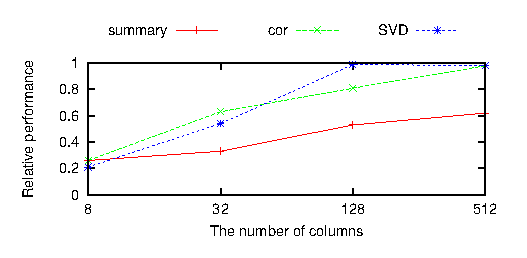
\includegraphics{FlashMatrix_figs/IM-vs-EM-stat.eps}
		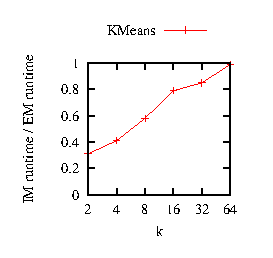
\includegraphics{FlashMatrix_figs/IM-vs-EM-clust.eps}
		\vspace{-10pt}
		\caption{The relative runtime of FlashR in memory versus on SSDs
		on a dataset with $n=100M$ while varying $p$ (the number of features)
		on the left and varying $k$ (the number of clusters) on the right.}
		\label{perf:stat}
	\end{center}
  \vspace{-15pt}
\end{figure}

As the number of features or clusters increases, the performance gap between
in-memory and external-memory execution narrows and the external-memory
performance approaches in-memory performance for correlation and k-means
but not Naive Bayes (Figure \ref{perf:stat}). This observation conforms with
the computation and I/O complexity of the algorithms in Table \ref{tbl:algs}.
For correlation and k-means, the number of clusters or features causes computation
to grow more quickly than I/O, driving performance toward a computation bound.
% When the number of features
%gets larger, the computation of matrix multiplication in
%correlation and SVD grows more rapidly than I/O and eventually CPU becomes
%the bottleneck. The current implementation of correlation requires an additional
%pass on the input matrix to compute column-wise mean values, which results in
%lower external-memory performance. Similarly, as the number of clusters
%increases, the computation of k-means and GMM increases rapidly and
%these algorithms are dominated by their CPU computation as the number
%of clusters gets larger.
The computation bound is realized on few features or clusters for an I/O throughput
of 10GB/s. Because most of the machine learning algorithms in Table \ref{tbl:algs} have
computation complexities that grow quadratically with $p$, we expect FlashR on SSDs to
achieve the same performance as in memory on datasets with a higher dimension size.

%\begin{figure}
%	\begin{center}
%		\footnotesize
%		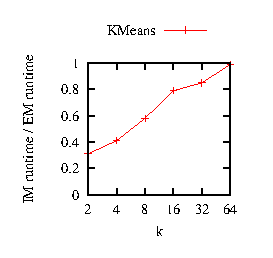
\includegraphics{FlashMatrix_figs/IM-vs-EM-clust.eps}
%		\caption{{\em Clustering} scaleup: FlashMatrix performance on SSDs
%      normalized to in-memory performance as the number of clusters vary.
%%      KMeans operates on the \rb{Friendster32} matrix and GMM on the
%%			by its performance in memory. As the number of clusters increases,
%%			the external-memory performance of these implementations approach
%%			to their in-memory performance.}
%}
%		\label{perf:clust}
%	\end{center}
%\end{figure}

\subsection{Effectiveness of optimizations}
We illustrate the effectiveness of our memory optimizations in FlashR for
DAG materialization.
We focus on two main optimizations: matrix operation fusion in main memory
to reduce data movement between SSDs and main memory (mem-fuse), and matrix
operation fusion in CPU cache to reduce data movement between main memory and
CPU cache (cache-fuse). Due to the limit of space, we only illustrate their
effectiveness when FlashR runs on SSDs.

Both optimizations have significant performance improvement on all algorithms
(Figure \ref{perf:em_opts}). Operation fusion in main memory (mem-fuse) achieves
substantial performance improvement in most algorithms, even in GMM,
which has the highest asymptotic computation complexity.
This indicates that materializing every matrix operation
separately causes SSDs to be the main bottleneck in the system and
fusing matrix operations in memory significantly reduces I/O.
Operation fusion in the CPU cache (cache-fuse) has significant impact
on the algorithms that are more complex and less bottlenecked by I/O.
This demonstrates that memory bandwidth is a limiting performance factor
once I/O is optimized.

\begin{figure}
	\begin{center}
		\footnotesize
		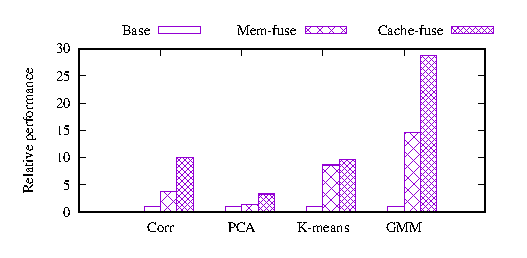
\includegraphics{FlashMatrix_figs/opts-EM.eps}
		\vspace{-10pt}
		\caption{The speedup by the optimizations in FlashR over the base
		implementation for different machine learning algorithms running on SSDs.
		The speedup is relative to the base implementation, which does not have
		optimizations to fuse matrix operations. The optimizations are applied
		to FlashR incrementally.}
		\label{perf:em_opts}
	\end{center}
  \vspace{-15pt}
\end{figure}


\section{Conclusions}
We present FlashMatrix, a matrix-oriented programming framework for general
data analysis. FlashMatrix scales to large datasets by utilizing commodity SSDs.
It provides a high-level functional programming interface for users to write
data analysis algorithms in R and
executes the R implementations in parallel and out of core automatically.
For simplicity and generality, the core of FlashMatrix only implements
a small number of generalized matrix operators (GenOps). It reimplements
many matrix operations in R \textit{base} package with GenOps to provide
a familiar programming environment to users. To improve performance,
FlashMatrix uses vectorized user-defined functions (VUDFs) to reduce the
overhead of function calls and fuses matrix operations to reduce data movement
between CPU and SSDs.

We demonstrate that the matrix-oriented functional programming interface in
FlashMatrix can achieve high performance and scalability for many data analysis
algorithms. We implement multiple statistics and
machine learning algorithms in R and compare their performance with Spark
MLlib, a high-optimized parallel machine learning library, on large datasets.
The R implementations executed in FlashMatrix significantly outperforms
the implementations in Spark MLlib. We further demonstrate that
the FlashMatrix implementations running in a single thread can outperform
the C and FORTRAN implementations in the R framework. The FlashMatrix
implementations also achieve linear speedup with multithreading.

Even though SSDs are still an order of magnitude slower than DRAM, the external-memory
execution of many data analysis algorithms in FlashMatrix can achieve performance
comparable to their in-memory execution. We demonstrate that an I/O throughput
of 10 GB/s is able to saturate CPU for many applications, even in a large parallel
NUMA machine. As such, the external-memory execution also benefits from many in-memory
optimizations.

FlashMatrix simplifies significantly the programming effort of writing
parallel and out-of-core implementations for large-scale data analysis. It
provides domain experts a familiar programming environment for implementing
their algorithms designed to process large datasets. It also significantly
increases productivity of writing an efficient implementation with performance
comparable to low-level programming languages. We believe FlashMatrix opens
a new opportunity for large-scale data analysis.


\section{Acknowledgement}
NSF Grant \# 1649880

%% Bibliography
{\footnotesize \bibliographystyle{acm}
\bibliography{kdd17}}


%\bibliography{bibfile}

\end{document}
